%             Exemple d'utilisation de la classe thesul
%             ------------------------------------------
%
%
% (de manière generale, les commandes de thesul sont celles
% qui ne sont pas complètement en minuscules)
%
% Voir la documentation complète pour plus de détails.
%   
%
% D. Roegel, 30 mars 2013
%
% \documentclass[12pt, oneside]{TUL/thesul}
\documentclass[12pt]{TUL/thesul}
%----------------------------------------------------------------------
%                     Chargement de quelques packages
%----------------------------------------------------------------------

% Si l'on veut produire une version PDF avec des hyperliens :
% \usepackage[pageanchor=false]{TUL/tulhypref}
% \usepackage[hidelinks, pdftex]{TUL/tulhypref}
\usepackage[hidelinks]{TUL/tulhypref}
% \usepackage[sc]{mathpazo}
\linespread{1.0}
% Si on veut le style de bibliographie named :
%\usepackage{named}

% Pour les figures :
\usepackage{graphicx}

% Si on veut des mini-tables des matières (utiliser minitoc-hyper 
% en conjonction avec tulhypref) :
\usepackage[french]{minitoc}

\usepackage{titlesec}
\usepackage{url}
\usepackage{listings}
\usepackage{pstricks}
\usepackage{subfigure}
\usepackage{amsmath}
\usepackage{amsthm}
\usepackage{amssymb}
\usepackage{tabularx}
\usepackage{textcomp}
\usepackage{multirow}
\usepackage[algoruled,french,onelanguage,algochapter]{algorithm2e}
\usepackage[section]{placeins}
\usepackage{xcolor}
\usepackage{colortbl}

\usepackage{epstopdf}
\usepackage{graphicx} % pour insérer des images
\usepackage{stmaryrd}
\usepackage{amsfonts}
% \usepackage{tikz}
% \usepackage{tikz-qtree}
% les figure imbriquées
\usepackage{epsfig}
% \usepackage{enumerate}

\usepackage{pgf}
\usepackage{tikz, calc}
% \usepackage{tikz-cd}
\usetikzlibrary{positioning}
\usetikzlibrary{fit}
\usetikzlibrary{shapes.multipart,calc}
\usetikzlibrary{arrows}

% \usepackage[math]{iwona} 
% \usepackage{iwona} 
% \SetMathAlphabet{\mathtt}{iwona}{OT1}{\ttdefault}{m}{n}

\usepackage[backend=biber, language=french, maxnames=5, citestyle=alphabetic,bibstyle=alphabetic,backref,abbreviate=false,dateabbrev=false,isbn=false,url=false,doi=true]{biblatex}
% \usepackage[backend=biber, language=french, maxnames=5,backref,abbreviate=false,dateabbrev=false,isbn=false,url=false,doi=true]{biblatex}
\addbibresource{these.bib}
% \usepackage[font=small,skip=0pt]{caption}
\usepackage[skip=0pt]{caption}
\usepackage{etoolbox}
\usepackage{needspace}

% Todo
\newcommand{\done}[1]{\todo[color=green!80!blue!80]{#1}}
\newcommand{\idone}[1]{\todo[inline,color=green!80!blue!80]{#1}}

% Samples
\newcommand{\telock}{tELock}

% Structure
\newtheorem{pb}{Problème}
\newtheorem{theo}{Théorème}
\newtheorem{defi}{Définition}
\newtheorem{prop}{Proposition}
\newtheorem{propri}{Propriété}
\newtheorem{pr}{Preuve}
\newtheorem{cor}{Corollaire}
\newtheorem{rem}{Remarque}
% \theoremstyle{remark}\newtheorem*{preuve}{Preuve}

% % Abbreviations :
\newcommand{\helloworld}{\texttt{Hello World}}
\newcommand{\nasm}{NASM}
\newcommand{\xq}{x86}
\newcommand{\xs}{x86$\_$64}

% Adresses mémoire :
\newcommand{\adr}[1]{$#1$}

% Registres
\newcommand{\eax}{\texttt{eax}}
\newcommand{\ebx}{\texttt{ebx}}
\newcommand{\ecx}{\texttt{ecx}}
\newcommand{\edi}{\texttt{edi}}

% Instructions
\newcommand{\mov}{\texttt{mov}}
\newcommand{\cmp}{\texttt{cmp}}
\newcommand{\add}{\texttt{add}}
\newcommand{\jmp}{\texttt{jmp}}
\newcommand{\ret}{\texttt{ret}}
\newcommand{\call}{\texttt{call}}
\newcommand{\push}{\texttt{push}}
\newcommand{\jne}{\texttt{jne}}
\newcommand{\je}{\texttt{je}}
\newcommand{\sub}{\texttt{sub}}

% Sémantique statique
\newcommand{\BN}{\mathbb N}
\newcommand{\BV}{\mathbb V}
\newcommand{\BX}{\mathbb X}
\newcommand{\BA}{\mathbb A}
\newcommand{\BP}{\mathbb P}
\newcommand{\BT}{\mathbb T}
\newcommand{\BL}{\mathbb L}
\newcommand{\BB}{\mathbb B}
\newcommand{\BNB}{\mathbb N\cup\{\bot\}}
\newcommand{\PN}{\mathcal{P}(\BN)}
\newcommand{\PMN}{\mathcal{P}_M(\BN)}
\newcommand{\Trs}{\mathbb N\cup\{\bot,\top\}}
\newcommand{\TTrs}{\mathcal P(\mathbb V\rightarrow\mathbb N\cup\{\bot,\top\})}
\newcommand{\Tr}{\PN\cup{\top,\bot}}
\newcommand{\TrM}{\PMN\cup\{\top,\bot\}}
\newcommand{\si}{\sigma_{init}}
\newcommand{\specialcell}[2][c]{%
  \begin{tabular}[#1]{@{}l@{}}#2\end{tabular}}
  
% Sémantique dynamique
\newcommand{\CA}{\mathcal A}
\newcommand{\CI}{\mathcal I}
\newcommand{\CC}{\mathcal C}
\newcommand{\CR}{\mathcal R}
\newcommand{\CW}{\mathcal W}
\newcommand{\da}[1]{$\CA[#1]$}
\newcommand{\di}[1]{$\CI[#1]$}
\newcommand{\dc}[1]{$\CC[#1]$}
\newcommand{\dr}[1]{$\CR[#1]$}
\newcommand{\dw}[1]{$\CW[#1]$}


\DefineBibliographyStrings{french}{
        in = {},%
%       in = {\emph{Dans}}%
        backrefpage = {cité page},
        backrefpages = {cité pages}
}

\titleformat{\chapter}[display]
  {\bfseries\huge}
  {\filleft\Large\chaptertitlename~\thechapter}
  {1ex}
  {\titlerule\vspace{1.5ex}\filright}
  [\vspace{1ex}\titlerule]

%-------------------------------------------------------------------
%                             Marges
%-------------------------------------------------------------------

% pour positionner les vraies marges:
%\SetRealMargins{1mm}{1mm}

%-------------------------------------------------------------------
%                             En-têtes
%-------------------------------------------------------------------

% Les en-têtes: quelques exemples
%\UppercaseHeadings 
%\UnderlineHeadings
%\newcommand\bfheadings[1]{{\bf #1}}
%\FormatHeadingsWith{\bfheadings}
%\FormatHeadingsWith{\uppercase}
%\FormatHeadingsWith{\underline}
\newcommand\upun[1]{\uppercase{\underline{\underline{#1}}}}
\FormatHeadingsWith\upun

\newcommand\itheadings[1]{\textit{#1}}
\FormatHeadingsWith{\itheadings}

% pour avoir un trait sous l'en-tete:
\setlength{\HeadRuleWidth}{0.4pt}

\usepackage[disable]{todonotes}

\begin{document}
\OddHead={{\leftmark\rightmark}{\hfil\slshape\rightmark}}
\EvenHead={{\leftmark}{{\slshape\leftmark}\hfil}}
\OddFoot={\hfil\thepage}
\EvenFoot={\thepage\hfil}
\pagestyle{ThesisHeadingsII}

\mainmatter 

% \chapter{Techniques d'obscurcissement de code}
% L'analyse d'un logiciel malveillant a pour but de comprendre ses mécanismes internes : selon les logiciels il peut, entre autres, s'agir des techniques d'attaque, de communication avec le concepteur ou d'autres programmes malveillants, de clés de chiffrement utilisées. Le programmeur a donc intérêt à protéger son logiciel contre l'analyse. Son but est de la rendre plus compliquée pour nécessiter plus de ressources en temps ou en argent de la part de l'analyste.

De nombreuses techniques de protection sont applicables à un programme binaire pour rendre son analyse plus compliquée. Certaines rendent le code plus difficile à comprendre en ajoutant par exemple du code inutile. Une autre technique consiste à modifier le programme au cours de son exécution afin que le code réellement utile du binaire ne soit pas lisible à première vue : on parle alors d'auto-modification.

Un auteur de programmes malveillants peut produire dans un premier temps son programme sans protection puis utiliser un logiciel de protection ou \emph{packer} qui produit un binaire sémantiquement équivalent mais qui est rendu plus difficile à analyser. En pratique l'exécutable final, protégé, combine plusieurs techniques d'obscurcissement dont des techniques d'auto-modification.

Dans ce chapitre nous chercherons rapidement a comprendre les difficultés rencontrées pour quiconque cherche à protéger son programme contre l'analyse. Dans un second temps nous nous intéresserons aux protections rencontrées lors de l'analyse de logiciels malveillants et en particulier aux problèmes liés au chevauchement de code assembleur et à l'auto-modification.

% Nous décrivons maintenant plusieurs techniques d'obscurcissement statiques ainsi que l'auto-modification.

% $\mathcal{T}$

\section{Théorie de l'obscurcissement}
\itodo{Chaîner les protections}

Collberg et Nagra \cite{nagra2009surreptitious} définissent plusieurs propriétés souhaitables pour une protection logicielle, nous reprenons ici quelque uns de leurs arguments. La première propriété est que le programme protégé soit équivalent en terme de sorties que le programme d'origine.
Une protection, ou obscurcissement, d'un programme P est une transformation $\mathcal{T}$ telle que le programme $\mathcal{T}(P)$ a le même comportement que P : quelle que soit l'entrée I de P, $\mathcal{T}(P)(I)=P(I)$.
On souhaite également ne pas affecter de manière importante les performances du programme, que ce soit en termes de temps d'exécution ou de taille des binaires.

Afin d'évaluer l'efficacité des protections il est nécessaire de définir les actifs que l'on cherche à protéger. 
Il peut s'agir de quelques algorithmes centraux au programme, de clé de chiffrement, du nom des fonctions et des variables utilisées, etc.
Il est également utile de masquer l'utilisation de techniques de protection qui pourraient attirer l'attention lors d'une analyse antivirale. De même si l'analyste se doute que le binaire emploi des protections, il n'est pas souhaitable qu'il lui soit aisé d'identifier quelles méthodes sont employées. Ainsi dans les modifications apportées au programme il est préférable que le programme final ressemble à un programme qui aurait pu être compilé, par exemple en évitant d'utiliser des instructions exotiques rarement utilisées en pratique.


En pratique un auteur de logiciel malveillant masque les symboles utiles à l'analyse tels le nom des fonctions à la compilation. Il est utile que le vecteur de propagation réussisse à masquer qu'il est protégé, s'il l'est, pour éviter une détection prématurée par un antivirus. La charge finale et les éventuels mécanismes de communication sont eux protégés contre l'analyse.\todo{cite}

\section{Exemples d'obscurcissement}
De nombreuses techniques d'obscurcissement sont utilisées en pratique, nous en donnons quelques exemples ici.

\paragraph{Insertion de code mort.}
Insérer du non atteignable (ou code mort) peut forcer un désassembleur par parcours linéaire à se désaligner avec le code réellement exécuté et à favoriser le code mort au détriment du code légitime.
L'exemple donné en figure \ref{fig:junk_right} montre de l'assembleur avec deux octets de données placés à la suite d'un instruction \jmp. Ces deux octets aux adresses $0x08048062$ et $0x08048063$ ne sont pas atteignables. Pourtant un désassembleur linéaire (Figure \ref{fig:junk_fooled}) chercherait à les désassembler et serait alors incapable de voir une partie des instructions réellement exécutées.


\begin{figure}
\begin{lstlisting}[language={[x86masm]Assembler}, escapechar=~]
08048060    eb 02               jmp 0x8048064
08048062    0a 05		~(code non atteignable)~
08048064    83 f9 02            cmp ecx, 0x2
08048067    74 00               je 0x8048069
08048069    bb 02 00 00 00      mov ebx, 0x2 ;  0x00000002
\end{lstlisting}
\caption{Insertion de code mort dans du code légitime}
\label{fig:junk_right}
\end{figure}

\begin{figure}
\begin{lstlisting}[language={[x86masm]Assembler}, escapechar=~]
08048060    eb 02               jmp 0x8048064
08048062    0a 05 83 f9 02 74   or al, [0x7402f983]
08048068    00 bb 02 00 00 00   add [ebx+0x2], bh
\end{lstlisting}
\caption{L'insertion de code mort dupe facilement un désassemblage par parcours linéaire}
\label{fig:junk_fooled}
\end{figure}

\FloatBarrier

\paragraph{Appels de fonctions sans retour.}
L'utilisation d'un contrôle de flot non standard peut forcer un désassembleur par parcours récursif à explorer du code non atteignable. 
Le comportement par défaut de l'instruction \call\ à une adresse $a$ et de taille $n$ est d'empiler l'adresse de retour $a+n$ puis de sauter vers la première adresse de la fonction appelée.
L'instruction \ret\ placée à la fin de la fonction appelée dépile la première valeur de la pile et provoque un saut vers celle-ci.

Normalement la valeur dépilée lors du \ret\ est $a+n$ afin que le flot d'exécution revienne à la fonction appelant.
Ainsi un désassembleur récursif désassemble à partir de la cible du \call\ ainsi que de l'adresse de retour.

Une technique classique d'obscurcissement \cite{LD03}\cite{PMA} consiste à combiner l'empilement d'une adresse (\push\ $a$) et l'instruction \ret. Ces deux instructions provoquent un saut vers l'adresse $a$ sans possibilité de revenir à l'instruction suivant le \call. La transformation consiste alors à remplacer des instructions \jmp\ par la séquence \push\ puis \ret\ puisque les deux suites d'instructions suivantes sont équivalentes.
\begin{center}
\begin{tabular}{c|c}
\push\ \adr{a} & \jmp\ \adr{a}\\
\ret &
\end{tabular}
\end{center}

\paragraph{Prédicats opaques.}
% À l'instar de son comportement avec une instruction \call, 
Lorsqu'un désassembleur récursif rencontre une instruction de saut conditionnel comme \je, qui provoque un saut si les deux valeurs comparées sont égales, il cherche à désassembler à la fois la cible potentielle du saut comme l'instruction suivante, qui sera exécutée si la condition n'est pas remplie.
Une autre technique courante d'obscurcissement consiste à utiliser comme condition du saut une relation que le programmeur sait toujours vraie ou fausse \cite{MKK07}. De cette manière il prédit qu'une seule des deux branches est atteignable alors qu'un désassembleur va parcourir également la branche inutile.
Une telle condition est appelée un prédicat opaque et peut par exemple être implémentée par des relations d'arithmétique. Par exemple en appliquant le petit théorème de Fermat \cite{fermat} : quel que soit l'entier e, $e^3\ =\ e\ mod\ 3$.
Le programmeur sait que l'égalité est toujours vérifiée mais un analyseur statique ne pourra pas le déterminer aisément.

\paragraph{Applatissement de graphe de flot de contrôle.}

\section{Chevauchement de code}
\itodo{citer PMA}
\itodo{biblio + complète}
\itodo{figure telock : les octets, jolis}
On a vu que la taille d'une instruction assembleur varie de un à 15 octets \done{15 dans intel2 chercher 15}.
De plus rien n'empêche que la cible d'un saut soit une adresse se trouvant être au milieu d'une autre instruction.
Ainsi on parle de chevauchement de code lorsque deux instructions (ou plus) à des adresses différentes sont codées sur des adresses communes. Si une instruction à l'adresse \adr{a} de taille $k\geq 2$ est atteignable, il peut y avoir une autre instruction valide et atteignable à l'adresse \adr{a+1} et ces deux instructions se chevauchent.

Il est à noter que, comme indiqué par Sikorski et Honig \cite{PMA}, il n'y a dans ce cas aucun désassemblage sous forme de liste d'instructions assembleur qui soit correct puisqu'une telle liste devra choisir entre l'instruction à l'adresse \adr{a} et celle à l'adresse \adr{a+1} alors qu'elles sont toutes les deux valides et atteignables. Une solution pour écrire un tel code assembleur est de mettre la première instruction en temps qu'instruction classique tandis que la deuxième sera présente sous forme d'octets codés en dur dans le fichier assembleur.

\paragraph{Exemple dans \telock.}
Le code de la figure \ref{fig:telock_obf_disas} est extrait d'un programme protégé par \telock\ désassemblé à l'aide d'un parcours récursif à partir de l'adresse \adr{01006e7a}. Il y a une instruction \texttt{jmp +1} à l'adresse \adr{01006e7d} et codée sur les deux octets \texttt{eb ff}, qui saute vers l'adresse \adr{01006e7d+1} où est présenté l'instruction \texttt{dec ecx}, codée sur \texttt{ff c9} et qui partage donc l'octet \texttt{ff} à l'adresse \adr{01006e7d+1} avec l'instruction \jmp.

Le code assembleur permettant d'être assemblé en ces octets est donné figure \ref{fig:telock_obf_asm} : la première instruction \jmp\ peut être présente dans le code tandis que l'instruction \dec\ la chevauchant est codée en dur grâce à l'octet \texttt{c9}.

\begin{figure}
% \scriptsize
% 0x01006e73    00 0c 0b        add [ebx+ecx], cl
% 0x01006e76    80 34 0b 67     xor byte [ebx+ecx], 0x67
\begin{lstlisting}[language={[x86masm]Assembler}, escapechar=~]
01006e7a    fe 04 0b        inc byte [ebx+ecx]
01006e7d    eb ff           jmp +1
01006e7e       ff c9        dec ecx
01006e80    7f e6           jg 01006e68
01006e82    8b c1           mov eax, ecx
\end{lstlisting}
% \end{framed}
\caption{Désassemblage récursif de \telock}
\label{fig:telock_obf_disas}
\end{figure}

\begin{figure}
% \scriptsize
% 0x01006e73    00 0c 0b        add [ebx+ecx], cl
% 0x01006e76    80 34 0b 67     xor byte [ebx+ecx], 0x67
\begin{lstlisting}[language={[x86masm]Assembler}, escapechar=~]
inc byte [ebx+ecx]
jmp +1
db c9 			; ajout de l'octet c9
jg 01006e68
mov eax, ecx
\end{lstlisting}
% \end{framed}
\caption{Code assembleur du chevauchement de \telock}
\label{fig:telock_obf_asm}
\end{figure}


Le graphe de flot de contrôle correct pour ce code est donné sur la figure \ref{fig:telock_cfg}. Le sommet orange est la première instruction et les lignes en pointillés reliant deux sommets marquent un chevauchement entre les instructions de ces sommets.

\begin{figure}
\begin{center}
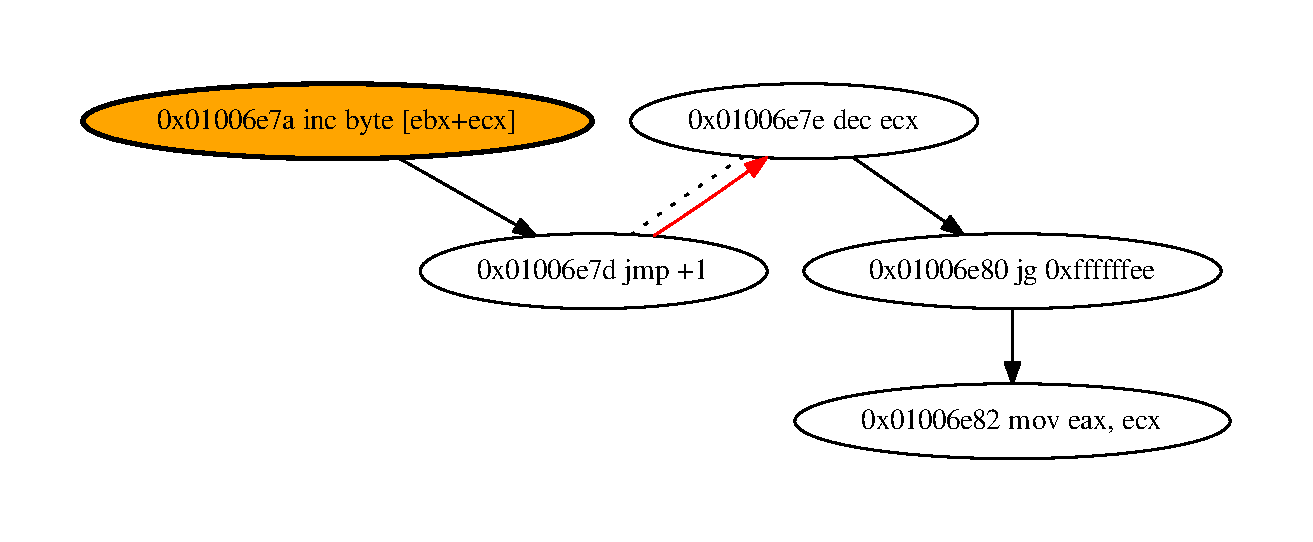
\includegraphics[width=0.8\textwidth]{supports/disasm/telock/telock.pdf}
\end{center}
\caption{Graphe de flot de contrôle de \telock}
\label{fig:telock_cfg}
\end{figure}

\paragraph{Exemple dans UPX.}

\section{Auto-modification}

% \begin{figure}
% \begin{center}
% \begin{tabular}{|l|l|l|}
% \hline
% Adresse & Octets & Instruction\\
% \hline
%  8048060  &  (...)         	& Pile -> RWX \\ 
%  804807c  &  bf 00 00 00 00         &  mov    edi, 0x0 \\
%  8048081  &  b8 91 80 04 08         &  mov    eax, 0x8048091 \\
%  8048086  &  66 c7 00 eb 00         &  mov    [eax], 0xeb \\
%  804808b  &  66 c7 40 01 07 00      &  mov    [eax+1], 0x7 \\
%  8048091  &  eb 0e                  &  jmp    80480a1 <edi3> \\
%  8048093  &  bf 01 00 00 00         &  mov    edi,0x1 \\
%  8048098  &  eb 0e                  &  jmp    80480a8 <fin> \\
%  804809a  &  bf 02 00 00 00         &  mov    edi,0x2 \\
%  804809f  &  eb 07                  &  jmp    80480a8 <fin> \\
%  80480a1  &  bf 03 00 00 00         &  mov    edi,0x3 \\
%  80480a6  &  eb 00                  &  jmp    80480a8 <fin> \\
%  80480a8  &  (...)		    &  Affiche edi \\
%  80480c3  &  (...)		    & Quitte \\
% \hline
% \end{tabular}
% \end{center}
% \caption{Exemple de code auto-modifiant}
% \label{fig:unevague_v0_code}
% \end{figure}

\begin{figure}
\begin{center}
\subfigure[Code assembleur]{
\begin{tabular}[b]{|l|l|l|}
\hline
Adresse & Octets & Instruction\\ 
\hline
 8048060  &  (...)         	& Pile -> RWX \\ 
 804807c  &  bf 00 00 00 00         &  mov    edi, 0x0 \\
 8048081  &  b8 91 80 04 08         &  mov    eax, 0x8048091 \\
 8048086  &  66 c7 00 eb 00         &  mov    [eax], 0xeb \\
 804808b  &  66 c7 40 01 07 00      &  mov    [eax+1], 0x7 \\
 8048091  &  eb 0e                  &  jmp    80480a1 <edi3> \\
 8048093  &  bf 01 00 00 00         &  mov    edi,0x1 \\
 8048098  &  eb 0e                  &  jmp    80480a8 <fin> \\
 804809a  &  bf 02 00 00 00         &  mov    edi,0x2 \\
 804809f  &  eb 07                  &  jmp    80480a8 <fin> \\
 80480a1  &  bf 03 00 00 00         &  mov    edi,0x3 \\
 80480a6  &  eb 00                  &  jmp    80480a8 <fin> \\
 80480a8  &  (...)		    &  Affiche edi \\
 80480c3  &  (...)		    & Quitte \\
\hline
\end{tabular}
\label{fig:unevague_v0_code}
}
\subfigure[Graphe de flot de contrôle]{
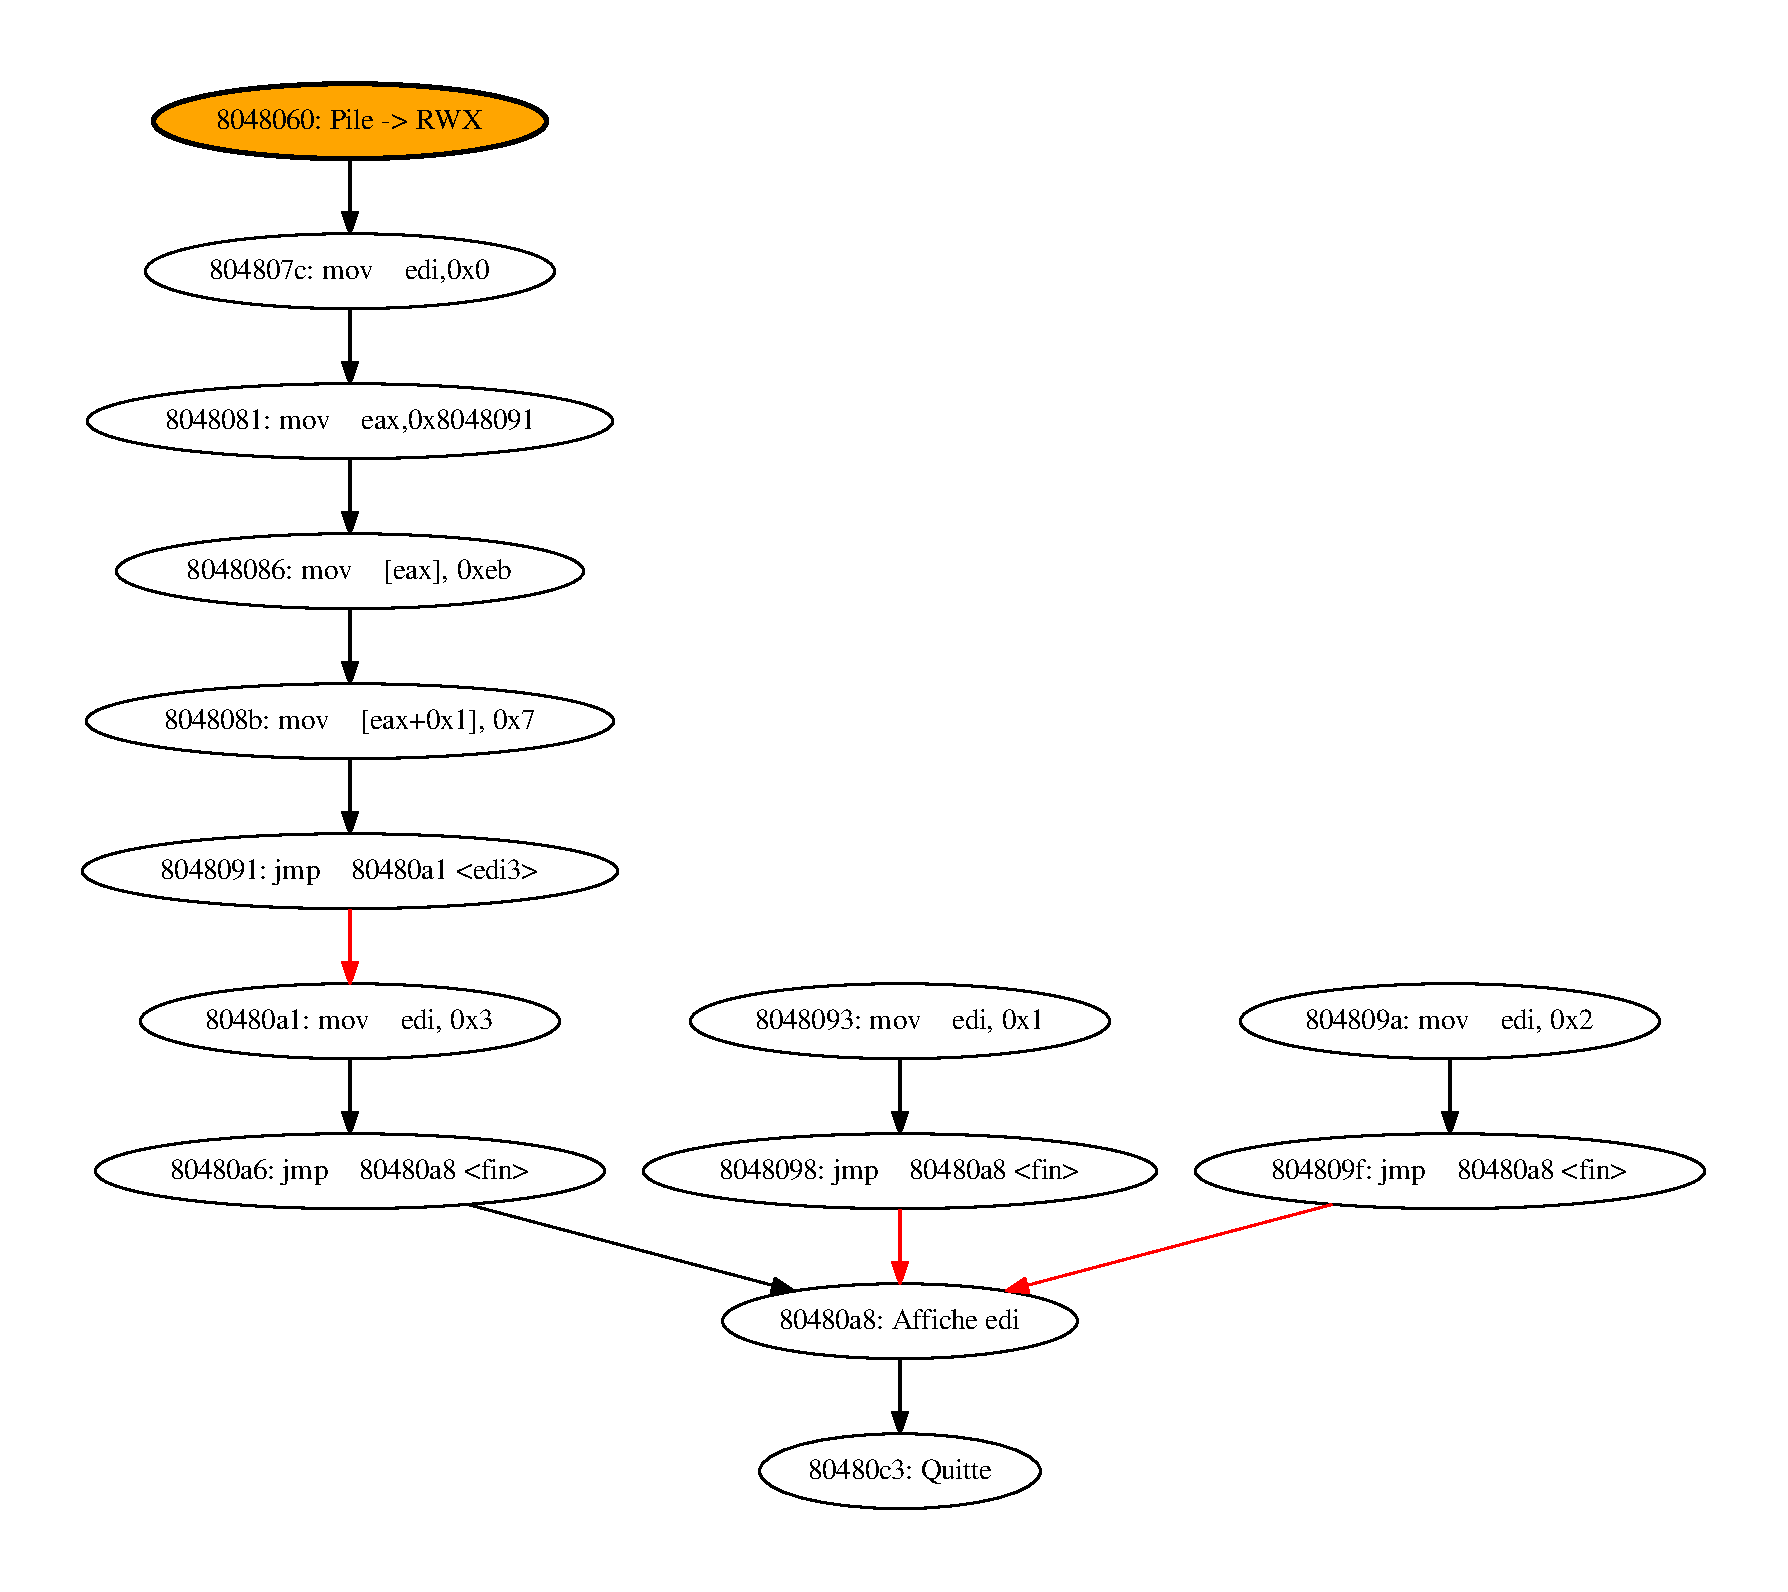
\includegraphics[width=1.0\textwidth]{supports/unevague/uv.pdf}
\label{fig:unevague_v0_cfg}
}
\end{center}
\ijym{détailler les ... (en annexe?)}
\ijym{fonction f, adresses f, f+1, f+3, ...}
\caption{Code assembleur auto-modifiant}
\label{fig:unevague_v0}
\end{figure}

Il a été expliqué dans la section \ref{section:assembleur} que, avec l'architecture de Harvard modifiée, le code n'est pas physiquement séparé des données lors de l'exécution sur une machine réelle.
Un programme auto-modifiant est simplement un programme utilisant cette propriété pour modifier le code assembleur le définissant au cours même de son exécution.
Ainsi on parle de comportement auto-modifiant lorsqu'une instruction du programme est codée sur au moins un octet qui a au préalable été modifié par ce programme.

En pratique les processeurs récents implémentent une protection, appelée bit NX ou W\textasciicircum X (prononcé ``W xor X''), permettant d'empêcher qu'une page mémoire puisse être à la fois écrite et exécutée lors de l'exécution du programme.
Cette protection a été ajoutée pour éviter des attaques résultant en l'exécution de code dans des données écrites par l'utilisateur du programme et non pour interdire l'auto-modification qui a des cas d'utilisation légitimes.
De ce fait l'activation ou non de la protection est spécifiée lors de la compilation et si un programme n'est pas protégé il lui suffit d'utiliser un appel système (\texttt{mprotect} sous linux) pour autoriser l'exécution de code sur la pile.

Prenons le programme de la figure \ref{fig:unevague_v0_code}. Ce programme commence par autoriser l'accès en écriture à la la section de code \ptext\ puis écrit sur la pile, modifie la valeur du registre \edi\ et termine par l'affichage de la valeur de \edi.
Si on ne prend pas en compte l'écriture sur la pile, il semble évident au vu du graphe de flot de contrôle (Figure \ref{fig:unevague_v0_cfg}), vu que la première instruction de saut provoque un saut vers l'instruction \texttt{mov edi,0x3} et que la seconde provoque l'affichage de \edi, que la valeur finale du registre est 3.
Pourtant les instructions \texttt{mov [eax],0xeb} et \texttt{mov [eax+1],0x07} aux l'adresse $0x8048086$ et $0x804808b$ remplacent le saut initial par un saut vers l'adresse $0x8048098$ où la valeur de \edi\ sera fixée à 2 avant l'affichage de celle-ci.


On constate ici que le programme se modifie au cours de son exécution et donc
\begin{itemize}
 \item On ne peut pas se contenter de la représentation d'origine du programme pour l'analyser.
 \item Le graphe de flot de contrôle initial peut être amené à évoluer au cours de l'exécution du programme.
\end{itemize}

\section{Logiciels malveillants et obscurcissement}
\itodo{packers, comment chaîner les obfuscations}
\itodo{utiliser des petites variations d'un packer pour éviter la détection, parler de la détection}

\section{Conclusion}
Cette thèse s'intéresse particulièrement à l'analyse des programmes écrits en assembleur \xq\ et \xs. Ces programmes ont en général été compilés à partir d'un langage de haut niveau puis ont été modifiés à l'aide d'un logiciel de protection. Les binaires que l'on étudie sont donc protégés avec des techniques statiques comme auto-modifiantes. Notre travail consiste alors à chercher à désassembler correctement ces programmes dans le but de faciliter leur analyse.

Les chapitres suivants détailleront plusieurs techniques d'analyse que nous avons appliquées. Nous nous intéresserons d'abord à l'aspect auto-modifiant des programmes et verrons comment l'analyse dynamique peut être utilisée pour reconstruire un modèle pour le programme auto-modifiant. Dans un second temps nous introduiront des techniques d'analyse statiques pour chercher à recomposer le maximum de code assembleur du programme et contourner d'autres méthodes de protection comme le chevauchement de code.

% \DontFrameThisInToc
\DontFrameThisInToc
\chapter*{Conclusion et perspectives\label{chap:conclusion}}
\section*{Synthèse des travaux réalisés}
% \itodo{pb 0: analyse de programmes obfusqués}
% \itodo{pb 1: analyse du chevauchement de code}
% \itodo{pb 2: analyse/désassemblage des programmes sms}

Notre contribution à l’analyse de programmes obscurcis s'est concentrée sur l'analyse de deux techniques de protection : l'auto-modification et le chevauchement de code.
Nous avons décrit un langage assembleur disposant d’une sémantique concrète compatible avec l’exécution de programmes auto-modifiants.
Nous avons étendu BAP, une plateforme d’analyse de binaires existante, pour lui permettre d’évaluer des programmes auto-modifiants et de séparer des programmes simples en différentes vagues d'exécution.
Nous avons formalisé le problème du chevauchement de code et étudié l’usage que les programmes obscurcis font de cette méthode de protection. 
Enfin nous avons proposé une technique de désassemblage consistant à effectuer une analyse dynamique que l’on complète à l’aide de techniques d’analyse statique. 
Cette technique a pour objectif de reconstruire un graphe de flot de contrôle dont nous avons défini la forme idéale.
Nous avons implémenté un détecteur réalisant l'analyse dynamique à l'aide de l'outil d'instrumentation Pin et reconstruisant le graphe de flot de contrôle paramétré par cette exécution.
La pertinence de cet outil a été démontrée lors de l'analyse de programmes obscurcis.

Notre contribution à l’analyse morphologique consiste en la formalisant du sous-problème d’isomorphisme de sous-graphes qu’elle cherche à résoudre.
Nous avons proposé une alternative à l'algorithme d'Ullmann, fonctionnant par recherche de parcours au sein d'un graphe de flot.
Cette approche est aussi précise que les approches existantes mais est beaucoup plus rapide. Nous l'avons implémentée et avons également décrit et implémenté un second algorithme, incorrect, mais dont le temps d’exécution constant ne dépend pas du nombre de programmes présents dans la base de détection.
Nous avons enfin proposé une application de la technique d’analyse morphologique au domaine de la détection de similarités logicielles \cite{REAT12,mal12} et appliqué cette méthode pour analyser quelques logiciels malveillants spécifiques dont Duqu et Stuxnet \cite{sstic13,mal13}.

% Les programmes malveillants obscurcis sont notre objet d'étude principal.
% Notre objectif principal a été le désassemblage et la reconstruction du graphe de flot de contrôle d'un programme malveillant obscurci.
% Nous cherchions à contrer particulièrement deux méthodes d'obscurcissement. 
% La première est l'auto-modification, technique permettant aux programmes de cacher leur charge utile et de ne la révéler que juste avant son exécution. La seconde est le chevauchement de code, permettant à plusieurs instructions d'être codées sur des adresses communes.
% 
% Nous avons proposé une méthode d'analyse hybride, se basant sur une trace d'exécution, permettant de guider l'analyse statique.
% La trace d'exécution est récupérée, comme dans les travaux de Reynaud \cite{Reynaud2010}, par une analyse dynamique qui découpe l'exécution en parties successives, non auto-modifiantes, du programme, ou vagues.
% La trace restreinte à une vague ne présente pas d'auto-modification, ce qui permet l'emploi de méthodes d'analyse statique sur chacune des vagues.
% Cette analyse statique fait une utilisation intensive des informations contenues dans la vague afin de guider son analyse.
% Elle reprend certaines techniques détaillées par Krügel \cite{KruegelRVV04} mais fonctionne sur des binaires utilisant le chevauchement de code et permet d'en mesurer utilisation : nous avons proposé une sémantique pour le chevauchement de code rangeant les instructions dans des couches de code au sein desquelles il n'y a pas de chevauchement.
% 
% Nous avons implémenté cette technique d'analyse hybride et validé des expériences précédentes, comme celles menées par Calvet  \cite{Calvet2013}, montrant l'utilisation presque systématique de l'auto-modification par les programmes malveillants.
% Nous avons mis en lumière l'utilisation occasionnelle du chevauchement de code par certains logiciels de protection de binaire et quelques familles de logiciels malveillants.
% \\
% 
% La seconde partie de notre travail a été centrée sur la détection de programmes malveillants et la technique d'analyse morphologique \cite{BKM08}, consistant à comparer les graphes de flot de contrôles de programmes connus pour être malveillants à celui du programme que l'on cherche à analyser.
% L'objectif a été de comprendre les mécanismes permettant d'améliorer les performances du détecteur sachant qu'il cherchait à résoudre un cas simplifié du problème NP-complet de l'isomorphisme de sous-graphes.
% 
% Nous avons proposé une formalisation du problème exactement résolu par l'analyse morphologique : il s'agit d'un problème plus simple que celui de l'isomorphisme de sous-graphes et pour lequel il existe des solutions en temps polynomial.
% Nous avons alors réalisé un algorithme de détection dont le temps d'exécution croît linéairement avec le nombre de programmes malveillants connus. Cet algorithme est complet : il résout exactement le problème posé par l'analyse morphologique.
% Nous avons également implémenté un algorithme incomplet mais dont le temps d'exécution ne dépend pas du nombre de programmes malveillants connus.
% \\
% 
% Enfin nous avons cherché à appliquer cette approche à des cas concrets d'analyse de programmes.
% Une possibilité consiste à utiliser l'analyse morphologique pour la détection de similarités logicielles et en particulier l'utilisation de bibliothèques logicielles.
% Nous avons illustré cette idée avec un logiciel malveillant, Waledac, et son emploi d'OpenSSL.
% Ces travaux ont été publiés à REcon \cite{REAT12} et Malware \cite{mal12}.
% 
% Cette idée a également été utilisée sur les programmes malveillants Duqu et Stuxnet dont nous avons montré qu'ils ont du code en commun.
% Dans une optique de détection nous nous sommes alors interrogés sur la possibilité de détecter Duqu connaissant Stuxnet et avons montré qu'il était nécessaire de surveiller l'exécution de Duqu pour réagir à l'injection d'un code en mémoire, code que le détecteur morphologique était capable de relier à Stuxnet.
% Ces travaux ont fait l'objet de publications à Malware \cite{mal13} et SSTIC \cite{sstic13}.



% \itodo{solution1: couches + étude de l'emploi de cette technique}
% \itodo{solution2: le GFC qu'on veut + analyse hybride avec solution 1 + implem + ça marche}

% \itodo{pb 3: détection}
% \itodo{solution3: (littérature) comparaison des GFCs !}

% \itodo{pb 4: comment détecter efficacement avec les GFC ? + optimisation}
% \itodo{solution4: formalisation + algos + efficaces en théorie et en pratique}

% \itodo{cas concrets ?}
% \itodo{analyse de librairies + duqu/stux}

\section*{Perspectives}
% \itodo{pb 0/1/2: interprêtation abstraite pour récupérer les vagues, éventuellement prédire la vague suivante}
L'analyse hybride que nous avons développée n'utilise que des techniques élémentaires d'analyse statique :
elle ne cherche pas à interpréter les instructions trouvées à chaque vague. 
Notre approche ne permet donc pas de gérer les sauts dynamiques qui n'ont pas été parcourus par l'exécution suivie lors de la phase d'analyse dynamique.
Nous voudrions utiliser des techniques d’interprétation abstraite pour reconstruire plus précisément les vagues et éventuellement être capables de déterminer les potentielles vagues suivantes à partir de la vague courante.
D'autre part nous nous sommes concentrés sur l'analyse d'une unique trace d'exécution pour approximer le graphe de flot de contrôle parfait : nous voudrions être capables d'incorporer plusieurs traces différentes dans l'analyse afin de couvrir plus de code potentiellement exécuté.

L'analyse morphologique produit des résultats prometteurs pour la détection de programmes malveillants et de similarités logicielles mais ne prend en compte dans les graphes de flot de contrôle que l'enchaînement des instructions. D'autres critères pourraient être intégrés dans ces graphes, traduisant l'utilisation de certaines méthodes d'obscurcissement : on pourrait ajouter les arcs entre deux sommets illustrant un chevauchement de code.
D'autre part nous avons vu que notre méthode réduit la complexité du problème à résoudre, le rendant polynomial, au prix d'une perte de flexibilité dans les résultats qu'elle produit.
En particulier, l'inversion de certaines branches  dans un graphe conduit à une non détection, ce qui n'aurait pas été le cas si l'on avait gardé le problème d'isomorphisme de sous-graphes.
Nous souhaiterions développer et analyser des techniques de réduction et de détection des graphes de flot de contrôle plus résistantes à ces modifications, afin d'être capables de détecter plus de programmes similaires sans trop perdre en vitesse de détection.
Il serait alors crucial d'étudier de manière détaillée la précision de notre technique de détection dans des réels cas d'utilisation ainsi que sa résistance à des techniques d'obscurcissement spécifiquement élaborées pour la déjouer.
Nous souhaiterions donc déterminer si notre modèle, avec ces modifications, permet de construire un détecteur de logiciels malveillants efficace, précis et rapide lors de la détection, capable de fonctionner sur l'ordinateur d'un utilisateur final.

% \itodo{pb 3: prendre en compte + de choses dans les GFC : chevauchements, liens entre vagues, etc ?}

% \itodo{pb 4: dans l'implem: prendre des sites de taille quelconque, aider à la constitution de listes blanches, prendre en compte certaines inversions}


% \onecolumn
% La bibliographie (comme d'habitude)
% \nocite{*}
% \bibliographystyle{unsrt}
% \bibliographystyle{named}
% \bibliography{these}
\printbibliography

\NumberAbstractPages
\begin{ThesisAbstract}
\newpage
  \begin{FrenchAbstract}
    Cette thèse porte en premier lieu sur l'analyse et le désassemblage de programmes malveillants utilisant certaines techniques d'obscurcissement telles que l'auto-modification et le chevauchement de code.
Les programmes malveillants trouvés dans la pratique utilisent massivement l'auto-modification pour cacher leur code utile à un analyste.
Nous proposons une technique d'analyse hybride qui utilise une trace d'exécution déterminée par analyse dynamique.
Cette analyse découpe le programme auto-modifiant en plusieurs sous-parties non auto-modifiantes que nous pouvons alors étudier par analyse statique en utilisant la trace comme guide.
Cette seconde analyse contourne d'autres techniques de protection comme le chevauchement de code afin de reconstruire le graphe de flot de contrôle du binaire analysé.

Nous étudions également un détecteur de programmes malveillants, fonctionnant par analyse morphologique : il compare les graphes de flot de contrôle d'un programme à analyser à ceux de programmes connus comme malveillants.
Nous proposons une formalisation de ce problème de comparaison de graphes, des algorithmes permettant de le résoudre efficacement et détaillons des cas concrets d'application à la détection de similarités logicielles.
    \KeyWords{programmes malveillants, auto-modification, graphe de flot de contrôle, comparaison de graphes}
  \end{FrenchAbstract}
  \begin{EnglishAbstract}
    This dissertation explores tactics for analysis and disassembly of malwares using some obfuscation techniques such as self-modification and code overlapping.
Most malwares found in the wild use self-modification in order to hide their payload from an analyst.
We propose an hybrid analysis which uses an execution trace derived from a dynamic analysis.
This analysis cuts the self-modifying binary into several non self-modifying parts that we can examine through a static analysis using the trace as a guide.
This second analysis circumvents more protection techniques such as code overlapping in order to recover the control flow graph of the studied binary.

Moreover we review a morphological malware detector which compares the control flow graph of the studied binary against those of known malwares.
We provide a formalization of this graph comparison problem along with efficient algorithms that solve it and a use case in the software similarity field.
    \KeyWords{malwares, self-modification, control flow graph, graph comparison}
  \end{EnglishAbstract}
\end{ThesisAbstract}
\end{document}


